%************************************************
\chapter{Hypotheses tests}\label{sec: tests}
%************************************************
\section{Normality tests and qq-plots}
Hypotheses tests \emph{against} the normal 
Gau\ss ian distribution can be performed 
starting with the \texttt{shapiro.test(values)}.
The sample size affects
the results of the normality test:
\begin{verbatim}
set.seed(1)
x <- rlnorm(20, 0 ,.4)
y <- rlnorm(100, 0, .4)

R: shapiro.test(x)
R: shapiro.test(y)

	        Shapiro-Wilk normality test

data:  x                      | data: y
W = 0.98049, p-value = 0.9403 | W = 0.91864, p-value = 1.193e-05
\end{verbatim}
In small sample sizes, even big departures from
normality are not detected. QQ-plots help us to
represent deviations from normality, as in the
example below:
\begin{verbatim}
R: mtcars[, .(p.value = shapiro.test(mpg)[2]), 
             by = "cyl"]

   cyl   p.value
1:   6 0.3251776
2:   4 0.2605931
3:   8 0.3228563

p <- ggplot(mtcars, aes(sample = mpg, colour = factor(cyl)))
p <- p + theme(panel.grid.major = element_blank(), 
               panel.grid.minor = element_blank(),
               panel.background = element_rect(fill = '#002b36'),
               axis.line = element_line(colour = "black"),
               legend.text=element_text(size=16),
               legend.title=element_blank(),
               axis.title.x = element_text(vjust=0, size=16),
               axis.title.y = element_text(vjust=1, size=16),
               plot.title   = element_text(vjust=1.5, size=20)) 
p <- p + stat_qq()
show(p)
\end{verbatim}
\begin{figure}[htbp]
 \centering
 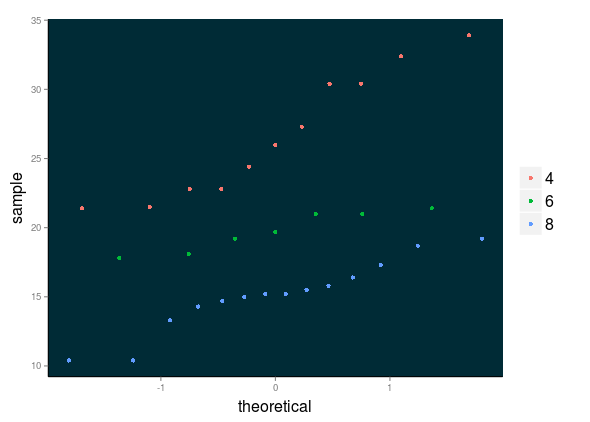
\includegraphics[scale=.6]{images/qqplots}
 \caption*{QQ-plot for data grouped by}
\end{figure}
Let us define a function that shows the rejection tests 
against the normal distribution for a set of 
grouped data, once an initial $p$-value is set.
\begin{verbatim}
shapiro.p.value <- function(my.column) {
    my.p.value <- '0.05'
    if(shapiro.test(my.column)[2] < my.p.value){
        return("rejected")
    } else {
        return("not rejected")
    }
} 
 
R: iris[, lapply(.SD, shapiro.p.value), by = Species]

      Species Sepal.Length  Sepal.Width Petal.Length  Petal.Width
1:     setosa not rejected not rejected not rejected not rejected
2: versicolor not rejected not rejected not rejected     rejected
3:  virginica not rejected not rejected not rejected not rejected
\end{verbatim}

\section{t-tests}
Student's t-test can be performed againts two 
sets of values to have the null hypothesis that their
means and variances to be the same, under the underlying 
assumption for both samples to come from a normal distribution.
If this were true, then the t-test statistic  
$t=\frac{(\bar{x}-\mu_0)}{(s/\sqrt{n})(\sigma/\sqrt{n})}$ would follow
a Student's t-distribution with $n_1 + n_2 -2$ degrees
of freedom, $n_1, n_2$ being the samples sizes.
For additional references, please see\footnote{ 
\url{http://statistics.berkeley.edu/computing/r-t-tests}
}
\medskip 

As an example we consider two normal samples and test 
the $t$-statistic obtained after $N$ t-tests. Given 
two sets of data $x, y$ then
\begin{verbatim}
set.seed(1)
tt <- t.test(rnorm(10), rnorm(10))

R: tt

	Welch Two Sample t-test

data:  rnorm(10) and rnorm(10)
t = -0.27858, df = 16.469, p-value = 0.784
alternative hypothesis: true difference 
in means is not equal to 0
95 percent confidence interval:
 -1.0022169  0.7689325
sample estimates:
mean of x mean of y 
0.1322028 0.2488450 

R: names(tt)
[1] "statistic"   "parameter"   "p.value"     "conf.int"       
[6] "estimate" "null.value"  "alternative" "method"      
[10] "data.name"
\end{verbatim}
where we are interested in the \texttt{statistic} parameter.
Therefore
\begin{verbatim}
    N <- 10000
tstat <- replicate(N, t.test(rnorm(10),rnorm(10))$statistic)

points <- seq(range(tstat)[1], range(tstat)[2], length=100)

# theoretical values of the t-distribution
theory <- dt(points, df = 10+10-2)  
# density values of the obtained t-statistics.
num    <- density(tstat, n=100)$y

data   <- data.table(points = points, theory = theory,
                     num = num)

p <- ggplot(data, aes(x=points))
p <- p + theme(panel.grid.major = element_blank(), 
               panel.grid.minor = element_blank(),
               panel.background = element_rect(fill = '#002b36'),
               axis.line = element_line(colour = "black"),
               legend.text=element_text(size=16),
               legend.title=element_blank(),
               axis.title.x = element_text(vjust=0, size=16),
               axis.title.y = element_text(vjust=1, size=16),
               plot.title   = element_text(vjust=1.5, size=20)) 
p <- p + geom_line(aes(y=theory, colour = "theory"))
p <- p + geom_line(aes(y=num, colour = "data"))
p <- p + scale_colour_manual(values=c("#2aa198","#268bd2"))
p <- p + labs(title = "t-test statistics")
p <- p + labs(y = "densities")
show(p)  
\end{verbatim}
\begin{figure}[htbp]
 \centering
 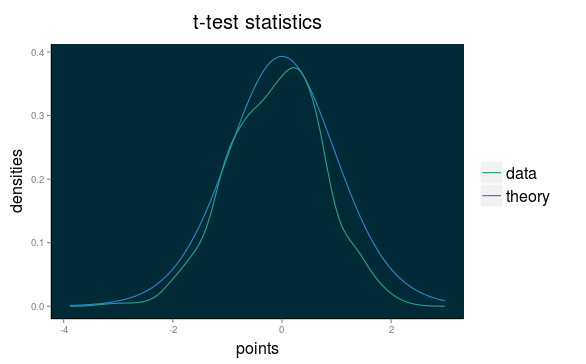
\includegraphics[scale=.6]{images/t_test}
 \caption*{$t$-test statistics densities}
\end{figure}
Another way to compare two densities is with 
a quantile-quantile plot. In this type of plot 
the quantiles of two samples are calculated at 
a variety of points in the range 
$\mathopen[0,1\mathopen]$, 
and then are plotted against each other. If the 
two samples came from the same distribution with 
the same parameters, we would see a straight line through 
the origin with unit slope; in other words, we are 
testing to see if various quantiles of the data are 
identical in the two samples. If the two samples came 
from similar distributions, but their parameters were 
different, we would still see a straight line, 
but not through the origin.
\bigskip

We will get \texttt{qqplot} to perform the necessary
calculations and then use \texttt{ggplot2} to 
display them.
\begin{verbatim}
x <- rnorm(100)
y <- rnorm(100)

dt <- as.data.table(qqplot(x, y, plot.it=FALSE))

p <- ggplot(dt)
p <- p + theme(panel.grid.major = element_blank(), 
               panel.grid.minor = element_blank(),
               panel.background = element_rect(fill = '#002b36'),
               axis.line = element_line(colour = "black"),
               legend.text=element_text(size=16),
               legend.title=element_blank(),
               axis.title.x = element_text(vjust=0, size=16),
               axis.title.y = element_text(vjust=1, size=16),
               plot.title   = element_text(vjust=1.5, size=20)) 
p <- p + geom_point(aes(x=x, y=y, colour = "QQ-plot"))
p <- p + geom_abline(aes(colour="ideal"), 
                     intercept = 0, slope = 1)
p <- p + scale_colour_manual(values=c("#2aa198","#268bd2"))
p <- p + labs(title = "t-test statistics")
p <- p + labs(y = "densities")
show(p)  
\end{verbatim}
\begin{figure}[htbp]
 \centering
 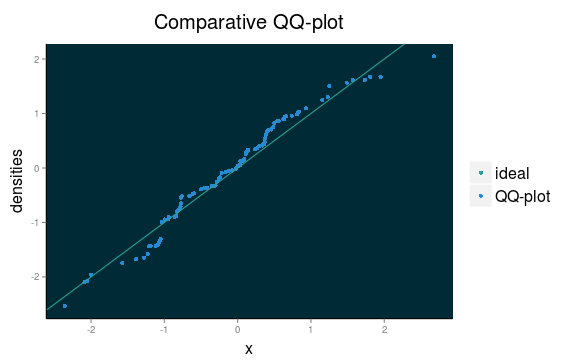
\includegraphics[scale=.6]{images/two_distr_qq}
 \caption*{QQ-plots to compare two distributions}
\end{figure}
Equivalently, if the null hypothesis were true,
namely if the two sets of data came from the 
same distribution, the $p$-value distribution
would be uniform. Doing so on the above analysis
we have
\begin{verbatim}
     N <- 10000
tpstat <- replicate(N,t.test(rnorm(10),rnorm(10))$p.value)
points <- seq(range(tpstat)[1], range(tpstat)[2], length=100)
# density values of the obtained p-values.
num    <- density(tpstat, n=100)$y
data   <- data.table(points = points, num = num)
\end{verbatim}
\begin{figure}[htbp]
 \centering
 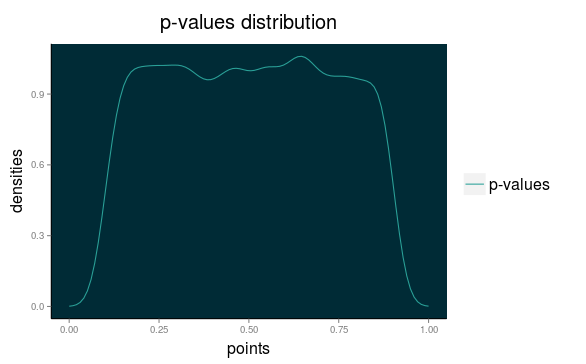
\includegraphics[scale=.6]{images/p_value_distr}
 \caption*{$p$-value uniform distribution}
\end{figure}

\section{Kruskal-Wallist test}
A collection of data samples are independent 
if they come from unrelated populations and 
the samples do not affect each other. Using the 
Kruskal-Wallis Test, we can decide whether the 
population distributions are identical without 
assuming them to follow the normal distribution.
\bigskip 

As a matter of example we can test 
whether the petal width in the \texttt{iris}
data set come from different distributions,
according the species. The null hypothesis 
is that they are identical populations:
\begin{verbatim}
R: kruskal.test(Petal.Width ~ Species, data = iris)

	Kruskal-Wallis rank sum test

data:  Petal.Width by Species
Kruskal-Wallis chi-squared = 131.19, df = 2, p-value < 2.2e-16
\end{verbatim}
It is therefore very \emph{unlikely} ($p$-value $<0.05$) 
the populations are identical.

\section{Dunn's test}

After having found out that a certain sets of data
come from dissimilar distributions, it is
possible to pairwise compare them to realise
which specific couplings disturb the entire set.
The above is obtained by means of the Dunn's test.
\begin{verbatim}
R: dunn.test(iris$Sepal.Width, g = iris$Species)

        Kruskal-Wallis rank sum test

data: x and group
Kruskal-Wallis chi-squared = 63.5711, df = 2, p-value = 0


              Comparison of x by group                            
                (No adjustment)                                
Col Mean-|
Row Mean |     setosa   versicol
---------+----------------------
versicol |   7.787706
         |     0.0000
         |
virginic |   5.374419  -2.413287
         |     0.0000     0.0079

R: dunn.test(iris$Sepal.Width, g = iris$Species)$P

[1] 3.411812e-15 3.841494e-08 7.904669e-03
\end{verbatim}
The pairwise $p$-values are smaller than any 
threshold, hence all three groups come from
three dissimilar populations.




